% !TEX root = ../MasterThesis.tex
\chapter{Verification}
\label{chap:verification}

Verification asks whether the candidate certificate
$\cert$ satisfies the drift condition everywhere on the domain
(Definition~\ref{def:verification}). Each method answers this question in its own way, and the methods differ sharply in what they demand and what they return.
We group them into three families. \emph{Symbolic} methods encode the
certificate and the dynamics exactly and search for a violating assignment; they
need full white-box access and struggle with scaling. 
\emph{Abstract interpretation} propagates sound over-approximations of the
network through each layer; it requires a computation graph for the condition of interest. A spectrum of methods allows tuning between tightness and speed. \emph{Sampling}
methods evaluate the drift only at points, so they work for black-box
dynamics, at the cost of a probabilistic rather than exact guarantee.

\section{Symbolic Solvers}

With symbolic methods, the main challenge is encoding. We require full, white-box access in order to precisely encode each constraint. This includes full access to the underlying dynamic system, including any noise, and the candidate certificate.

Symbolic methods feature heavily in deterministic verification settings
\cite{katz2017reluplex, abate2020lyapunov, peruffo2020barrier, abate2021fossil}; supermartingales, however, require the encoding of an expected value. For discrete noise distributions this is manageable: one enumerates the outcomes and takes the weighted average. In many cases, however, the noise is continuous, and no finite formula represents its expectation exactly. In this case, we employ a common strategy of discretising the noise pdf and over-approximating it in order to soundly reason over it
~\cite{lechner2022stability, zikelic2023reachavoid}.


\subsection{SMT}

Satisfiability Modulo Theories (SMT) directly extends Boolean satisfiability (SAT), the problem of finding a truth assignment satisfying a propositional formula. By allowing variables to range over richer domains governed by background theories such as nonlinear real arithmetic, we seek to find a satisfying assignment. In our context, we look for an assignment satisfying the negation of the supermartingale condition; it is this assignment that forms a counterexample.
\[
\exists x \in \aX : \drift(x) > 0
\]

We use Z3 as our SMT backend
\cite{demoura2008z3}. The ReLU certificate is piecewise-linear, so it
encodes exactly: each neuron becomes a case split, and the expected value in the
drift is a weighted sum over the noise branches. Z3 reasons in exact arithmetic
\cite{jovanovic2012nlsat},
so when it returns a verdict there is no numerical slack to worry about.

Z3's nonlinear real arithmetic is a sound and complete decision
procedure for polynomial constraints, so quadratic and even cubic dynamics such
as those in $\mathrm{DoubleWell}$ are handled exactly. The main difficulty lies in scalability.
Even on minimal problems (such as a tiny trained network of two layers of four neurons), Z3 frequently returns \emph{unknown} or exhausts its time budget (3600s).

Compounding this, continuous noise cannot be represented exactly, but it can be soundly over-approximated by binning it into a finite set
of branches with a conservative encoding whose slack shrinks as the number of bins
grows. This also grows the number of variables that Z3 must check, worsening the scalability wall above.

In addition, Z3 cannot handle transcendental relationships, which restricts both the dynamics we can certify ($\mathrm{Pendulum}$ system requires $\sin(x)$) and the certificates we can check (no sigmoid or tanh network architecture). Tools built on $\delta$-complete decision procedures, such as dReal
\cite{gao2013dreal}, can reason over these transcendental functions, but only up to a user-specified numerical error rather than exactly.

\subsection{MILP}

Mixed Integer Linear Programming (MILP) extends beyond satisfiability to optimisation problems. By combining propositions and numerical constraints, we represent the verification problem as maximising the drift $\drift$ (see Chapter~\ref{chap:refutation} for more details on defining optimisation problems), and if there exists a solution greater than 0, we reject the candidate.

We use Gurobi (version 13.0.1, via \texttt{gurobipy}) as our MILP backend
\cite{gurobi2026manual}. Casting verification as an optimisation
rather than a satisfiability query has a practical benefit: the solver returns
the worst-case drift as a number, so we learn not just \emph{whether} the
certificate fails but by how much. The $\relu$ certificate encodes with the usual
indicator and max constraints.

As with SMT, polynomial dynamics remain within reach, even though the tool is designed for piecewise-linear problems.

Enabling Gurobi's nonconvex mode turns it into a spatial branch-and-bound solver: it encloses each
product term in a convex relaxation and refines the variable ranges until the
relaxation is tight, converging to the global optimum. This is what lets it
verify the cubic $\mathrm{DoubleWell}$ exactly. One caveat
unique to Gurobi is that it works in floating point, so its guarantee holds only up
to the solver's numerical tolerances. Otherwise, the model grows with the network width and
the number of noise bins, echoing the scalability issues of SMT. As before, transcendental dynamics remain out of scope. Noise is handled exactly as in the SMT case: discrete outcomes enumerated,
continuous noise binned into a sound over-approximation.

The number of bins used to discretise the noise distribution is the crux of the
method's behaviour on stochastic dynamics. Writing $b$ for the
bins per noise dimension and $d_w$ for the dimension of the noise variable $w$, the expectation $\expectation$ is over-approximated
by $b^{d_w}$ cells, each carrying its own copy of the successor-network encoding,
so the program grows as $b^{d_w}$ (Figure~\ref{fig:milp_size}). With too few bins the over-approximation is so loose
that its drift exceeds the threshold even for a valid certificate: the
maximiser returns \emph{phantom} counterexamples --- a state whose true expected
drift is negative but whose binned over-approximation is positive --- and the CEGIS
loop is sent chasing a violation that does not exist. With too many bins the $b^{d_w}$
network copies make the program so large that the solver can no longer close the
optimality gap within the time budget. Only an intermediate \emph{window}
of $b$ both tightens the over-approximation enough to certify and stays small enough to
solve.


\begin{figure}[t]
  \centering
  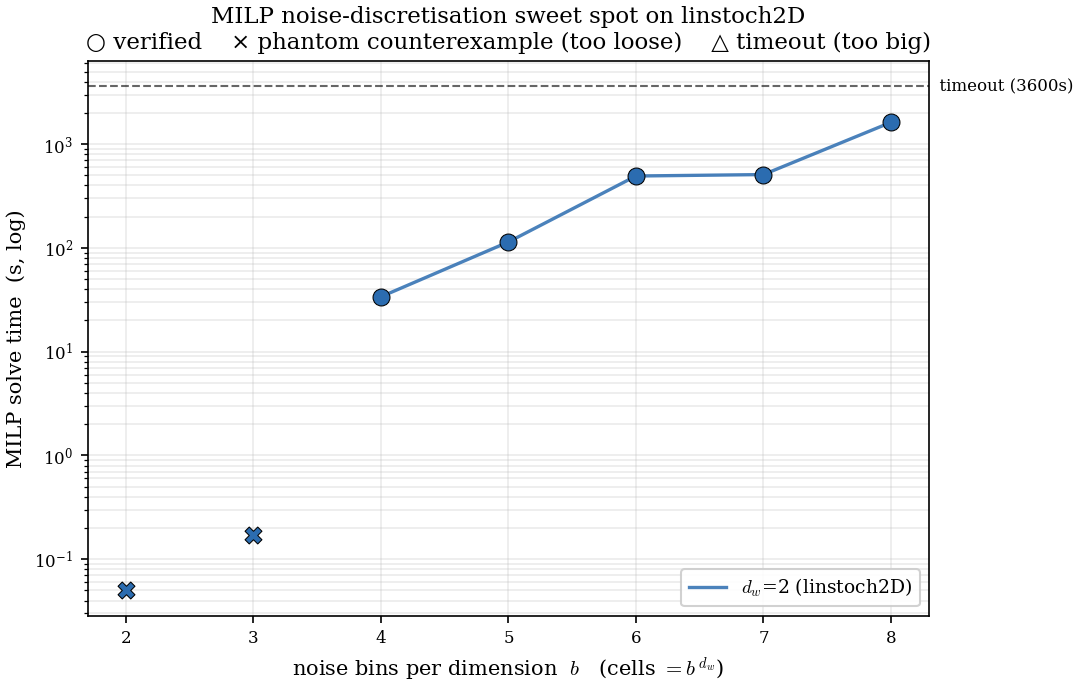
\includegraphics[width=0.85\textwidth]{Figures/milp_noise_disc.png}
  \caption{MILP verification of a stochastic-linear certificate on the
    two-dimensional $\mathrm{LinStoch}$ system, against the noise discretisation
    $b$ (bins per noise dimension, so the model carries $b^{d_w}$ noise cells).
    The \emph{phantom} regime below $b = 4$ and the steep growth in solve time
    above it (the cell count itself grows as $b^{2}$) are discussed in the text.}
  \label{fig:milp_nd}
\end{figure}

\begin{figure}[t]
  \centering
  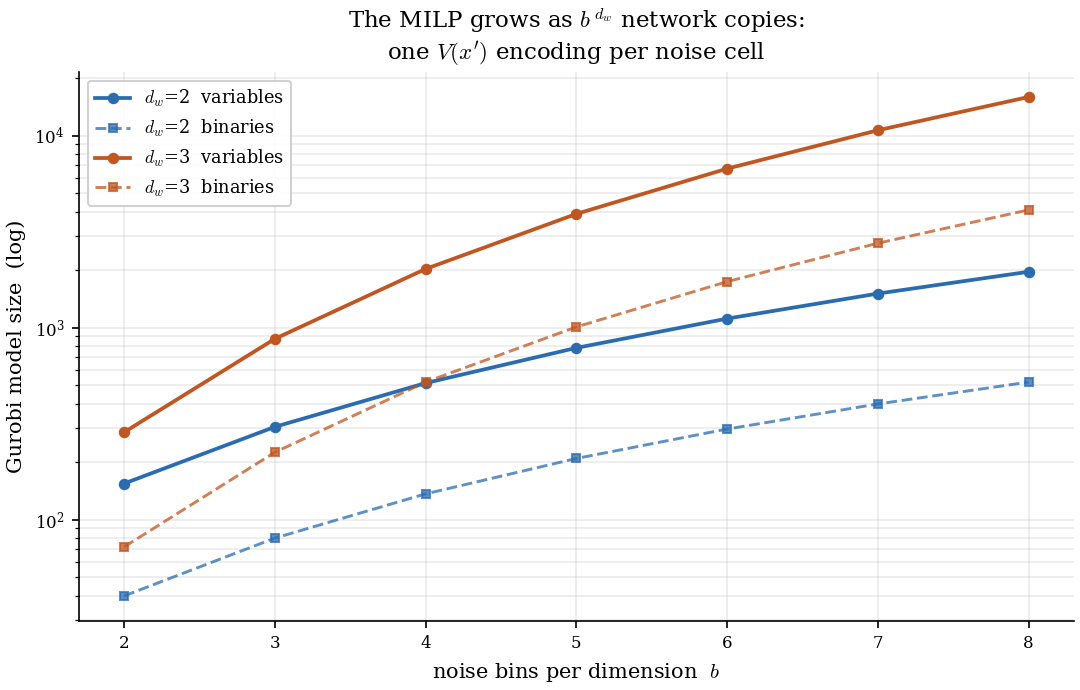
\includegraphics[width=0.7\textwidth]{Figures/milp_problem_size.png}
  \caption{The Gurobi model size (decision variables and
    binaries) grows as $b^{d_w}$, since each of the $b^{d_w}$ noise cells must represent and optimise over its
    own copy of the successor-network encoding. Tightening the
    over-approximation (larger $b$) and staying solvable are therefore in direct
    conflict, and the conflict is exponential in the noise dimension $d_w$.}
  \label{fig:milp_size}
\end{figure}

Figure~\ref{fig:milp_nd} traces this behaviour on $\mathrm{LinStoch}$ in two
dimensions. Below $b = 4$ the over-approximation is so loose that every candidate is
rejected by a phantom counterexample; from $b = 4$ onward the certificate verifies.
The cell count grows as $b^{2}$, and the solve time climbs far faster still, from $34$\,s
at $b = 4$ to some $27$ minutes at $b = 8$. No bin count in the swept range exhausts
the one-hour budget, so in two dimensions the binding constraint is the phantom
threshold below, not a timeout above.

The window nonetheless closes with dimension. Because the cell count is $b^{d_w}$, the
same sweep in three noise dimensions never escapes the phantom regime: every bin count we
could solve, up to $b = 8$ ($512$ cells), still returns a phantom counterexample,
while the $b^{3}$ growth drives a single solve past $1600$\,s by $b = 7$. No bin count
is at once tight enough to certify and cheap enough to solve, so the exact route
stalls without ever producing a valid certificate. This places the exact route's limit
between two and three noise dimensions, consistent with the frontier the
stochastic-certificate literature places at a handful of
dimensions~\cite{badings2025logRASM, lechner2022stability}.



\section{Abstract Interpretation}
\label{sec: abstract-interpret}

Rather than encode the problem exactly, abstract interpretation
over-approximates it. Given an input region, we propagate \emph{bounds} through a computation graph, so that the true output is always guaranteed
to lie within the computed enclosure. This makes the method sound by
construction: if the enclosure of the drift stays below the threshold, no input
in the region can violate it. The price is looseness (the enclosure is wider
than the true reachable set), and the central trade-off is how much tightness we
are willing to pay for. % CITED-QUOTE (xu2020autolirpa): "by generalizing existing LiRPA algorithms such as CROWN to operate on general computational graphs."
We use the auto\_LiRPA framework \cite{xu2020autolirpa}, which spans this
spectrum from cheap interval bounds to tighter linear relaxations.


\subsection{Interval Propagation}

Interval bound propagation
\cite{gowal2018ibp} is the simplest instance: we carry an interval
$[\underline{z},\overline{z}]$ for each neuron and push it through the affine and
activation layers. It is cheap and unconditionally sound, but also the loosest
option. Because it tracks each neuron independently, it ignores the correlations
between them: every $\relu$ that straddles zero is relaxed in isolation, so the
intervals widen quickly with depth and width. On our trained certificates the
enclosure is usually too loose to verify without extensive splitting of the input
region.


\subsection{Linear Relaxation}

CROWN \cite{zhang2018crown} tightens this by propagating \emph{linear} bounds rather than intervals:
each neuron is bounded above and below by an affine function of the inputs, which
preserves the inter-neuron correlations (unlike IBP) and yields far
tighter enclosures at a moderate cost. Where a single pass is still too loose to
decide a region, we close the gap with branch-and-bound, splitting the region and
bounding each piece. Optimising the relaxation slopes of each neuron by gradient
ascent --- \emph{$\alpha$-CROWN} \cite{xu2021alphacrown} --- yields a still-tighter
bound at a higher per-call cost, and is the strongest of the three engines we use.
One practical wrinkle is that the bound-propagation library
only supports a fixed catalogue of operations, so a certificate's output
activation must be expressed in terms it recognises: our hard-sigmoid activation function, for
instance, is decomposed into a scaling and a clamp. Figure~\ref{fig:box-evolution}
shows this branch-and-bound partition evolving on the $\mathrm{Pendulum}$
certificate, each cell shaded by whether its sound enclosure has yet cleared the
threshold.

\begin{figure}[htbp]
\centering
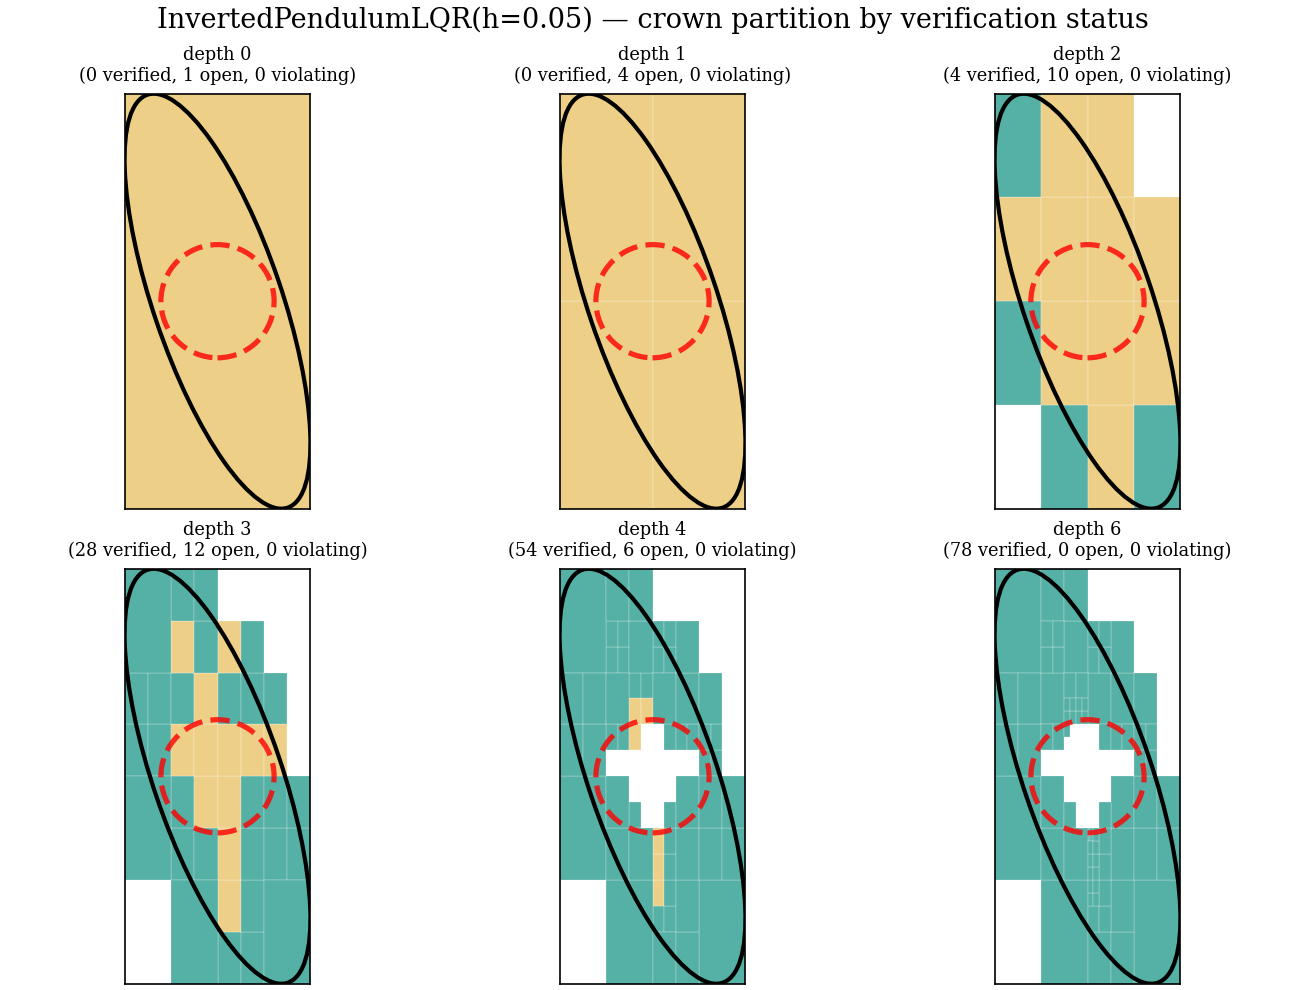
\includegraphics[width=0.85\linewidth]{Figures/pendulum_lqr_crown_grid.png}
\caption{Branch-and-bound in action: CROWN's partition of the 2D $\mathrm{Pendulum}$
state space at successive depths, for a verified certificate. Each cell is shaded by
its sound status --- \emph{verified} (drift upper bound $\le 0$, teal),
\emph{undecided} (amber, still to be split), or \emph{violating} (red); the black
curve marks the domain boundary and the red dashed circle the goal region. From a
single undecided box, auto\_LiRPA repeatedly halves the cells it cannot yet decide
until the whole domain is verified. Tighter relaxations reach this state with far
fewer splits than IBP --- the compute that the anytime view of
Figure~\ref{fig:pendulum-anytime} prices.}
\label{fig:box-evolution}
\end{figure}

CROWN tools such as \texttt{jax\_verify} \cite{jax_verify} and auto\_LiRPA require noise to be over-approximated through binning, as with the symbolic methods. Furthermore, they are not natively designed to handle discrete noise, requiring the spawning of multiple separate process threads to evaluate.


\begin{figure}[htbp]
\centering
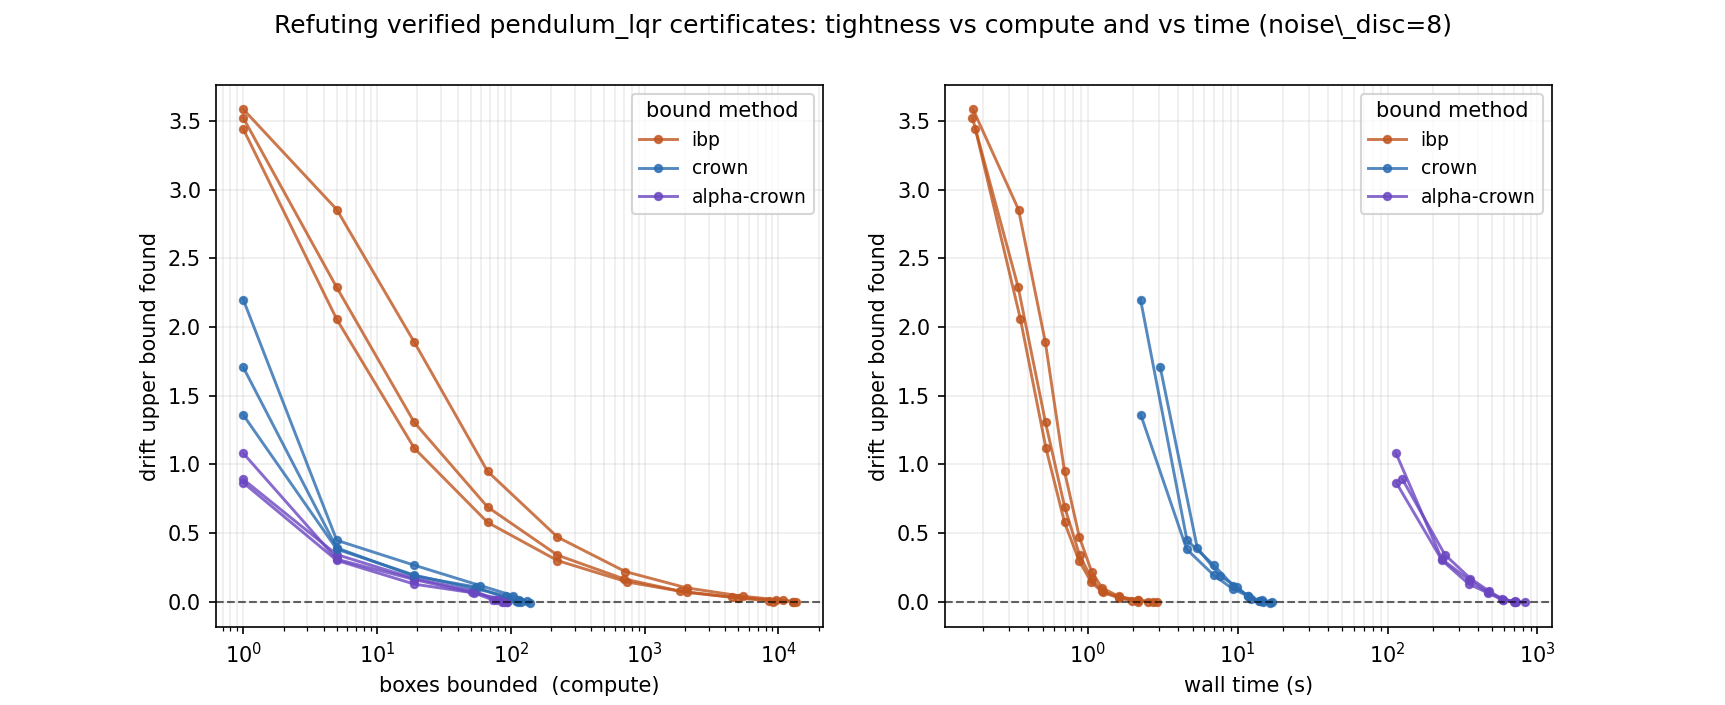
\includegraphics[width=0.82\linewidth]{Figures/pendulum_anytime.png}
\caption{Anytime tightness of the three bound-propagation engines on a verified
$\mathrm{Pendulum}$ certificate: the sound drift upper bound against wall-clock as
branch-and-bound refines. IBP is cheapest per unit compute but loosest, requiring the most domain partitions;
$\alpha$-CROWN reaches the tightest bound at the highest cost; CROWN sits between.
All three are sound at every step, as the bound only tightens.}
\label{fig:pendulum-anytime}
\end{figure}

\paragraph{Anytime Tightness.} Every engine in this family only ever \emph{tightens} its sound bound as
branch-and-bound refines, so it can be halted at any point and still return a
valid enclosure --- an \emph{anytime} guarantee that the drift $\drift$ exceeds the current upper bound nowhere. In particular, tighter bounding means less branching is required, and so fewer domain regions to check. Figure~\ref{fig:pendulum-anytime}
makes the resulting speed--tightness trade concrete on a verified
$\mathrm{Pendulum}$ certificate: IBP is the loosest at any compute budget, CROWN
tightens it, and $\alpha$-CROWN reaches the tightest bound at the highest cost.
This anytime soundness is precisely the property the CEGIS loop of
Chapter~\ref{chap:streamlining} exploits, since a verifier call can be stopped the
moment its bound crosses zero.





\section{Sampling}
\label{sec:sampling-methods}

Sampling methods sit at the opposite extreme from symbolic ones~\cite{zikelic2023reachavoid}.
They are the easiest to implement, since they need only sample
access to $\drift$: any form of noise or dynamics can be sampled without ever
representing its structure, and that flexibility is the whole appeal. The difficulty lies in providing a rigorous guarantee from finitely many points; an average over a
finite set of points says nothing about the gaps between them. What makes these
methods sound is a \emph{regularity} bridge, the drift-Lipschitz constant $L_\drift$, which
bounds how much the drift can change between samples; and even then the guarantee
is \emph{probabilistic}, holding with a chosen confidence $1-\delta$. For deeper discussion on estimating the Lipschitz constant, see Chapter~\ref{sec:lipschitz}. We discuss two methods below, a global Monte Carlo
estimate and an adaptive multi-armed-bandit search.

A sampling verifier evaluates $\drift$ only at finitely many points, so the
whole difficulty is bridging soundly from those points to the continuum between
them. Both methods below do so with a rigorous \emph{drift-Lipschitz} constant
$L_{\drift}$; as shown in Chapter~\ref{sec:lipschitz}, a valid choice is
$L_{\drift} = L_{\cert}\,(L_f+1)$, where we assume knowledge of a sound one-step Lipschitz constant of the dynamics $L_f$, and $L_{\cert}$ is a bound on the certificate's Lipschitz constant.

Each method relies on a simple concept: the confidence bound for a grid cell $B \in \mathcal{B}$ is derived from a statistical error as well as a discretisation error. The discretisation error is defined as the product of the diameter of $B$ and $L_\drift$, as we have seen before. The statistical error relies on Hoeffding bounds to estimate the confidence that the observed mean of the samples in $B$ reflects the true mean. This requires normalisation with respect to the range of values that $\drift$ can assume, which is non-trivial. To combat this, we restrict the class of $\cert_\theta$ that we can learn by constricting the output with either a clamp or a sigmoid activation. In our experiments, we clamp values in $[0,1]$ to avoid this normalisation step.

\subsection{Monte Carlo}
\label{sec:mc}

The Monte Carlo method is heavily inspired by the results and methods discussed in Chapter~\ref{sec:lipschitz}. We first discretise the domain uniformly according to $L_\drift$, and then take samples within each grid cell. We track the observed empirical mean of the drift on each cell $B$ and its statistical error to produce upper and lower confidence bounds. If the lower confidence bound for some $B$ is greater than zero, then we certifiably have a counterexample inside $B$. We return $B$ as a certified violating region and sample within it to supply the learner's next counterexamples. If the upper confidence bound is below zero, then we can certify that our certificate condition holds on $B$ with confidence $1-\delta$. If the process stalls, the discretisation error needs refinement, which motivates our next method.


% \paragraph{Underlying theory.}
% The natural sampling estimate of \eqref{eq:drift} is the \emph{average}
% exceedance $\mu = \expe_{X\sim\mathrm{Unif}(\aX)}[\max(0,\drift(X))]$,
% which a Hoeffding bound controls from finitely many draws. On its own this is
% \emph{unsound} as a verifier: the supremum we must bound is not controlled by
% the mean, because an arbitrarily thin violating spike contributes almost nothing
% to the average. Regularity is what closes the gap. If $\drift$ is $L_{\drift}$-Lipschitz a
% violation cannot be a spike: a point $x^\star$ with $\drift(x^\star)=\eta>0$ forces
% $\drift \ge \eta/2$ throughout the ball $\mathcal{B}(x^\star,\eta/2L_{\drift})$, so a large
% worst case necessarily inflates the average. This gives a quantitative exchange
% rate between the mean and the maximum.

% \begin{lemma}[Lipschitz mean-to-max]
% \label{lem:mc}
% Let $\drift$ be $L_{\drift}$-Lipschitz on $\aX\subset\RN^d$ and let
% $\mu = \expe_{X\sim\mathrm{Unif}(\aX)}[\max(0,\drift(X))]$. Then
% \begin{equation*}
%     \sup_{x\in\aX} \drift(x) \;\le\; \Phi(\mu),
%     \qquad
%     \Phi(\mu) := \Big(
%         \frac{2^{\,d+1}\, L_{\drift}^{\,d}\, \mathrm{Vol}(\aX)}{\kappa\, V_d}\, \mu
%     \Big)^{1/(d+1)},
% \end{equation*}
% where $V_d$ is the volume of the unit $d$-ball and $\kappa$ lower-bounds the
% fraction of a violation ball that lies inside $\aX$.
% \end{lemma}
% \medskip
% \noindent\textit{Proof sketch.}
% If $\eta:=\sup_x \drift(x)>0$ then $\drift\ge\eta/2$ on
% $\mathcal{B}(x^\star,\eta/2L_{\drift})\cap\aX$, whose volume is at least
% $\kappa\,V_d\,(\eta/2L_{\drift})^d$. Since $\max(0,\drift)\ge\eta/2$ there,
% $\mu \ge \tfrac{\kappa V_d}{2^{d+1}L_{\drift}^d\,\mathrm{Vol}(\aX)}\,\eta^{d+1}$;
% inverting for $\eta$ yields the bound.\hfill$\square$
% \medskip

% \paragraph{How it works.}
% The method is deliberately non-adaptive. It draws $n$ points uniformly from the
% working region, estimates the drift at each with $m$ successor samples of the
% inner expectation, and averages the exceedances to obtain $\widehat\mu$. A
% one-sided Hoeffding radius $r$ turns this into an upper confidence bound
% $\mu_{\mathrm{UB}} = \widehat\mu + r$ on the true mean $\mu$, valid with
% probability $1-\delta$. Lemma~\ref{lem:mc} then converts $\mu_{\mathrm{UB}}$ into
% a certified ceiling $\Phi(\mu_{\mathrm{UB}})$ on the worst-case drift. The nested
% inner estimate is harmless: $\max(0,\cdot)$ is convex, so by Jensen's inequality
% the noisy estimate over-shoots the true exceedance in expectation --- the safe
% direction for an upper bound. Finally, to look for a genuine counterexample the
% worst sampled point is re-evaluated with a large fresh batch of successor draws;
% only if its one-sided \emph{lower} confidence bound is positive is a violation
% reported, which prevents the maximum of many noisy estimates from being mistaken
% for a real one.

% \begin{algorithm}[H]
% \DontPrintSemicolon
% \KwIn{certificate $\cert$, dynamics sampler $f$, region $\aX$, margin
%   $\varepsilon$, confidence $\delta$, states $n$, inner draws $m$, drift-Lipschitz
%   $L_{\drift}$, value range $b$ (so $\cert\in[0,b]$), tolerance $\tau$}
% \KwOut{\textsc{Verified} / \textsc{Counterexample} / \textsc{Inconclusive}, and
%   a certified ceiling on $\sup_x \drift(x)$}
% $\kappa \leftarrow 2^{-d}$;\quad
% $\mathrm{Vol} \leftarrow$ volume of the bounding box of $\aX$;\quad
% $V_d \leftarrow \pi^{d/2}/\Gamma(\tfrac d2+1)$\;
% draw $x_1,\dots,x_n \sim \mathrm{Unif}(\aX)$\;
% \For{$i = 1,\dots,n$}{
%   $\widehat{\drift}_i \leftarrow \tfrac1m \sum_{j=1}^m \big[\cert(f(x_i,w_j)) - \cert(x_i) + \varepsilon\big]$
%   \tcp*{inner Monte Carlo}
% }
% $\widehat\mu \leftarrow \tfrac1n \sum_i \max(0,\widehat{\drift}_i)$;\quad
% $r \leftarrow (b+\varepsilon)\sqrt{\ln(1/\delta)/(2n)}$;\quad
% $\mu_{\mathrm{UB}} \leftarrow \widehat\mu + r$\;
% $\Phi \leftarrow \big(2^{d+1} L_{\drift}^{d}\,\mathrm{Vol}/(\kappa V_d)\cdot \mu_{\mathrm{UB}}\big)^{1/(d+1)}$
% \tcp*{Lemma~\ref{lem:mc}}
% $x^\star \leftarrow \arg\max_i \widehat{\drift}_i$;\quad re-estimate $\drift(x^\star)$ with a
% large fresh batch $\to$ lower bound $\ell$\;
% \lIf{$\ell > 0$}{\Return \textsc{Counterexample} $x^\star$}
% \lElseIf{$\Phi \le \tau$}{\Return \textsc{Verified} ($\sup_x \drift \le \tau$)}
% \lElse{\Return \textsc{Inconclusive} (ceiling $\Phi$)}
% \caption{Monte Carlo verifier (global Lipschitz mean-to-max)}
% \label{alg:mc}
% \end{algorithm}

% \paragraph{Requirements, strengths and limitations.}
% The method needs only \emph{sample} access to the dynamics --- it never encodes
% $f$ or $\cert$ --- together with a rigorous drift-Lipschitz bound $L_{\drift}$, a value
% range $b$ so that the exceedance is bounded, and the domain volume. Its strengths
% follow from that minimal interface: it is oblivious to the form of the noise and
% the dynamics, so continuous, discrete and transcendental systems are handled
% identically; it is embarrassingly parallel; and it is trivial to implement. Its
% weakness is the conversion in Lemma~\ref{lem:mc}. Reconstructing a
% $d$-dimensional volume back into a height costs the exponent $1/(d+1)$: with a
% Hoeffding radius $r\propto n^{-1/2}$ the certified ceiling shrinks only as
% $\Phi \propto n^{-1/(2(d+1))}$, so driving it below a tolerance $\tau$ requires on
% the order of $\tau^{-2(d+1)}$ samples. Crucially $\Phi(\mu_{\mathrm{UB}})$ is
% strictly positive for any finite budget (even with no sampled violation,
% $\mu_{\mathrm{UB}}$ equals the concentration radius), so the method can certify
% $\sup_x \drift \le \tau$ only for a \emph{positive} $\tau$ --- never $\sup_x \drift\le 0$
% outright.

% \paragraph{What it yields.}
% Algorithm~\ref{alg:mc} produces, with probability $1-\delta$, a sound numerical
% \emph{upper bound} on the worst-case drift over the entire region: a certified
% ceiling, not a binary verdict. It also returns genuine (re-confirmed)
% counterexamples when the certificate is violated. What it does \emph{not} give is
% a violating region --- the estimate is purely pointwise --- nor an exact proof.
% It is therefore best read as the sound-but-expensive baseline whose
% $\tau^{-2(d+1)}$ cost, and its inability to reach a zero tolerance, precisely
% motivate the adaptive method that follows.

\subsection{Multi-Armed Bandit}
\label{sec:mab}

We consider the Monte Carlo method to be non-adaptive: it samples uniformly in each grid cell, and the cells are uniformly sized. The Multi-Armed Bandit method seeks to improve on this through adaptive sampling and discretisation. We first consider the domain in its entirety and estimate its upper and lower confidence bounds on the mean drift. Similar termination rules apply; however, in the case where the confidence bound straddles zero (making our cell undecided), we consult the error bounds. If the discretisation error is greater than the statistical error, then we split the grid according to some fixed splitting rule. If the reverse is true, then we take more samples. With this, grid refinement is data-driven: grid cells with strong average decrease are verified early and can be pruned as potential violation locations.

Motivated by sample efficiency, in the case where multiple cells are undecided, we can check the top $k$ cells with the highest upper confidence bounds to act upon. With $k=1$, we take only the most unsure cell, where further sampling will be most beneficial. With larger $k$, we act upon more and more cells at once, approaching a more uniform gridding. We therefore see a tradeoff between sample-efficiency and time-efficiency through the parameter $k$.

\paragraph{Experimentation.} This method requires both tight estimation of $L_\drift$ and tight bounds on the statistical error. For our experiments, we used LipBaB (M2 in Section~\ref{sec:tightdrift}) and an empirical-Bernstein radius for the error bounding. Unfortunately, with loose bounds, we were unable to achieve termination within our sample budget ($10^9$ samples) for either method consistently on any benchmark.

\section{The Capability Boundary}
\label{sec:capability}

Across the suite the three families separate cleanly, and the boundary follows
the dynamics class and the noise dimension. The \emph{symbolic} engines are the
most precise where they apply but the least available: Z3, though a complete
decision procedure for the polynomial systems, returned \emph{unknown} or
exhausted its budget on essentially every trained-network round, and Gurobi's
exact route closes between two and three noise dimensions as the
discretisation window shuts (Figure~\ref{fig:milp_nd}); neither can encode the
$\mathrm{Pendulum}$'s transcendental dynamics, and both abstain there. The
\emph{sampling} verifiers are the most general in principle, indifferent to
the form of the noise and the dynamics, but sound worst-case sampling proved
too expensive in practice: within our budgets neither Monte Carlo nor the
multi-armed bandit could be driven to termination, so we do not carry them
forward as benchmarked engines. The \emph{bound-propagation} family has the
widest coverage and is the only one to reach the transcendental
$\mathrm{Pendulum}$ --- yet it is not universal either: $\mathrm{LinStoch}$,
whose noise-floor equilibrium leaves the relaxation little margin to work
with, was certified only by the exact MILP route inside its discretisation
window (Figure~\ref{fig:milp_nd}). No single family clears the whole suite;
the boundary is two-sided, with the exact route alone owning the additive-noise
linear system and bound propagation alone reaching past the symbolic frontier.
Within the LiRPA family, IBP, CROWN and $\alpha$-CROWN trade per-call
tightness against cost along the anytime curve of
Figure~\ref{fig:pendulum-anytime}.

This boundary fixes the cast for the remainder of the thesis. The three LiRPA
engines are the sound verifiers of the end-to-end synthesis campaign of
Chapter~\ref{chap:streamlining}, run on the three systems they certify, where their per-call costs (from
sub-second for IBP on $\mathrm{LinSwitch}$ to some twenty minutes for
$\alpha$-CROWN on the $\mathrm{Pendulum}$) are measured inside the loop.
And every round in which a verifier (MILP or LiRPA) rejected a candidate
leaves behind a genuine refutation problem; these rejected candidates form the
faux-certificate library on which Chapter~\ref{chap:refutation} benchmarks the
refuters. What no engine changes is the fundamental expense of a sound call,
which must reason over the entire domain; removing that cost from every round
of synthesis is the subject of the final chapter.

% \paragraph{Underlying theory.}
% The Monte Carlo verifier is \emph{global}: it reconstructs the worst case from a
% single average over the whole region, and Lemma~\ref{lem:mc} shows the price is a
% conversion no finite budget can drive to zero. The multi-armed-bandit (MAB)
% verifier removes that penalty by keeping the estimate \emph{local}. The region is
% covered by axis-aligned cells; on each cell $C$ we maintain a confidence interval
% on $\sup_{x\in C} \drift(x)$ that combines a statistical term, from the samples drawn
% in $C$, with a discretisation term, the cell diameter scaled by the
% drift-Lipschitz bound:
% \begin{equation}
% \label{eq:mab-ci}
%     \sup_{x\in C} \drift(x)
%     \;\le\;
%     \widehat m_C(n)
%     \;+\; \underbrace{L_{\drift}\,\mathrm{diam}(C)}_{\text{discretisation}}
%     \;+\; \underbrace{\mathrm{EB}_C(n)}_{\text{statistical}} .
% \end{equation}
% The statistical term is a \emph{stitched empirical-Bernstein} radius built from a
% predictable-variance estimate; it is valid simultaneously for all sample counts
% $n\ge 1$, so a cell may be sampled repeatedly without a union bound over $n$.
% Confidence is instead allocated across cells: the $j$-th cell that the search
% opens is given failure budget $\delta_C = 6\delta/(\pi^2 j^2)$, and since
% $\sum_{j\ge1} 6/(\pi^2 j^2)=1$ the \emph{total} failure probability over every
% cell ever opened is at most $\delta$.

% \begin{theorem}[Soundness]
% \label{thm:mab}
% With the opened-cell allocation $\delta_C = 6\delta/(\pi^2 j(C)^2)$ and the
% stitched empirical-Bernstein radius, with probability at least $1-\delta$,
% simultaneously for every opened cell $C$, every $n\ge 1$ and every $x\in C$,
% \begin{equation*}
%     \drift(x) \in \widehat m_C(n) \pm \big[\, L_{\drift}\,\mathrm{diam}(C) + \mathrm{EB}_C(n) \,\big].
% \end{equation*}
% Consequently, if every cell of a covering of $\aX$ has upper confidence
% bound at most $0$, then $\sup_{x\in\aX} \drift(x)\le 0$ with probability at
% least $1-\delta$; and if some cell has lower confidence bound above $0$, it
% contains a genuine violation.
% \end{theorem}

% \paragraph{How it works.}
% The search is an upper-confidence-bound bandit over cells. Each round it selects
% the $k$ live cells with the largest upper bound --- the ones most likely to still
% hide a violation --- draws a batch of samples in each, and folds them into that
% cell's running mean and predictable variance, from which the interval
% \eqref{eq:mab-ci} is recomputed. A cell whose upper bound has fallen to $0$ or
% below is \emph{proven safe} and retired; a cell whose lower bound has risen above
% $0$ is a \emph{counterexample} and halts the search. The remaining, undecided
% cells fall into two regimes. Where the statistical term still dominates, more
% samples will resolve the cell, so the bandit simply keeps selecting it. Where the
% discretisation term $L_{\drift}\,\mathrm{diam}(C)$ dominates, no amount of sampling can
% shrink the interval, so the cell is \emph{split}, halving its diameter and
% handing each child a fresh confidence budget. This is the source of the method's
% efficiency: regions with a comfortable margin are covered by a few large cells,
% and refinement is spent only where the margin is thin.

% \begin{algorithm}[H]
% \DontPrintSemicolon
% \KwIn{certificate $\cert$, dynamics sampler $f$, region $\aX$, margin
%   $\varepsilon$, confidence $\delta$, drift-Lipschitz $L_{\drift}$, batch width $k$,
%   budgets}
% \KwOut{\textsc{Verified} / \textsc{Counterexample} (with cell) /
%   \textsc{Inconclusive}}
% initialise the live set with a uniform grid over $\aX$; assign each cell
% an opening index $j$\;
% \While{budget remains}{
%   drop cells proven outside $\aX$ or inside the equilibrium\;
%   \lIf{all live cells have $\mathrm{UCB}\le 0$}{\Return \textsc{Verified}}
%   $\mathcal{S} \leftarrow$ the $k$ live cells with largest $\mathrm{UCB}$\;
%   \For{$C \in \mathcal{S}$}{
%     draw a batch of samples in $C$; update $\widehat m_C, \widehat V_C, n_C$
%     (predictable-centre statistics)\;
%     $\mathrm{UCB}_C \leftarrow \widehat m_C + L_{\drift}\,\mathrm{diam}(C) + \mathrm{EB}_C$;\quad
%     $\mathrm{LCB}_C \leftarrow \widehat m_C - L_{\drift}\,\mathrm{diam}(C) - \mathrm{EB}_C$\;
%   }
%   \lIf{$\exists\, C\in\mathcal{S}:\ \mathrm{LCB}_C > 0$}{\Return
%     \textsc{Counterexample} $C$}
%   retire every cell with $\mathrm{UCB}_C \le 0$ \tcp*{proven safe}
%   split every undecided cell whose discretisation term dominates; children
%   inherit the parent's samples and a fresh opening index\;
% }
% \Return \textsc{Inconclusive} (budget exhausted)\;
% \caption{Multi-armed-bandit verifier (adaptive stitched empirical-Bernstein)}
% \label{alg:mab}
% \end{algorithm}

% \paragraph{Requirements, strengths and limitations.}
% Like the Monte Carlo verifier, MAB needs only sample access to the dynamics, a
% rigorous $L_{\drift}$, and a bounded value range for the empirical-Bernstein term; it
% inherits the same indifference to the form of the noise and the dynamics. Its
% advantage is adaptivity: whereas a uniform covering would place cells at the
% finest resolution everywhere, MAB refines only along the thin-margin frontier, so
% in practice it opens far fewer cells than the worst-case count
% $\sim (L_{\drift}\,\mathrm{diam}(\aX)/\text{margin})^d$. The limitations are
% those of any sample-based worst-case method: the statistical radius is the honest
% cost of soundness, and cells pinned on a knife-edge margin demand many samples;
% the cell count still grows with dimension; and, as with Monte Carlo, a bounded
% certificate and a valid $L_{\drift}$ are prerequisites.

% \paragraph{What it yields.}
% Theorem~\ref{thm:mab} makes MAB a genuine \emph{formal verifier}: a run that
% retires every cell certifies $\sup_{x\in\aX} \drift(x)\le 0$ over the whole
% region with probability $1-\delta$ --- the exact drift condition, at a zero
% tolerance, which the global Monte Carlo method cannot reach. Beyond the binary
% verdict it returns genuine counterexamples and, unlike Monte Carlo, localises
% them: the offending \emph{cell} is a certified violating region, not just a
% point, which is exactly the information the counterexample-guided training loop
% consumes. The live set at termination is moreover a full state-space tiling,
% labelling each cell verified, unresolved, or unsafe, which makes the certificate
% inspectable rather than a single bit (Figure~\ref{fig:mab}).

% \begin{figure}[h]
% \centering
% 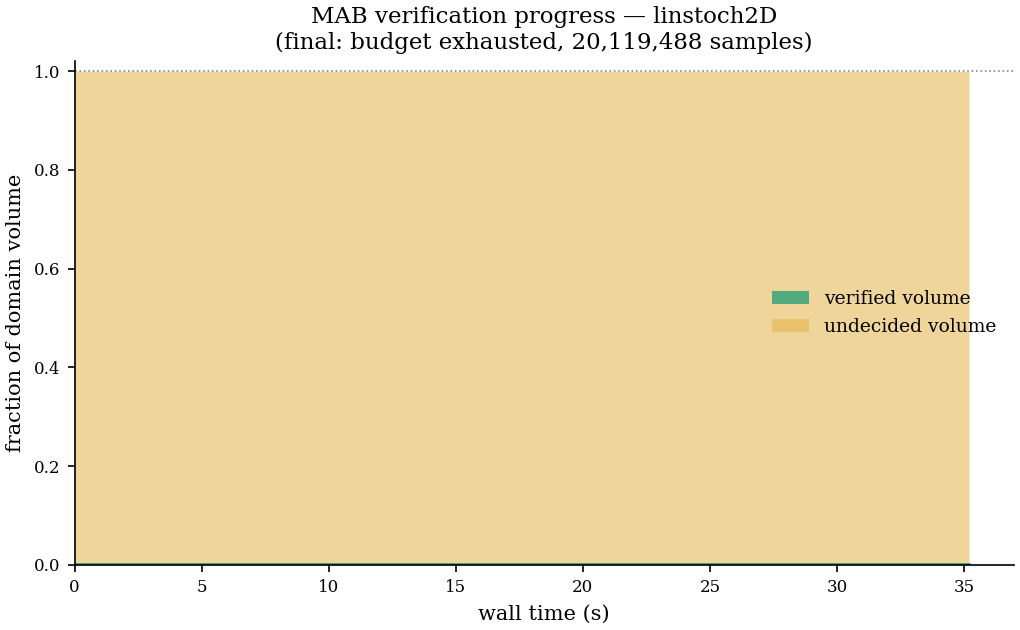
\includegraphics[width=0.49\linewidth]{Figures/mab_area.png}\hfill
% 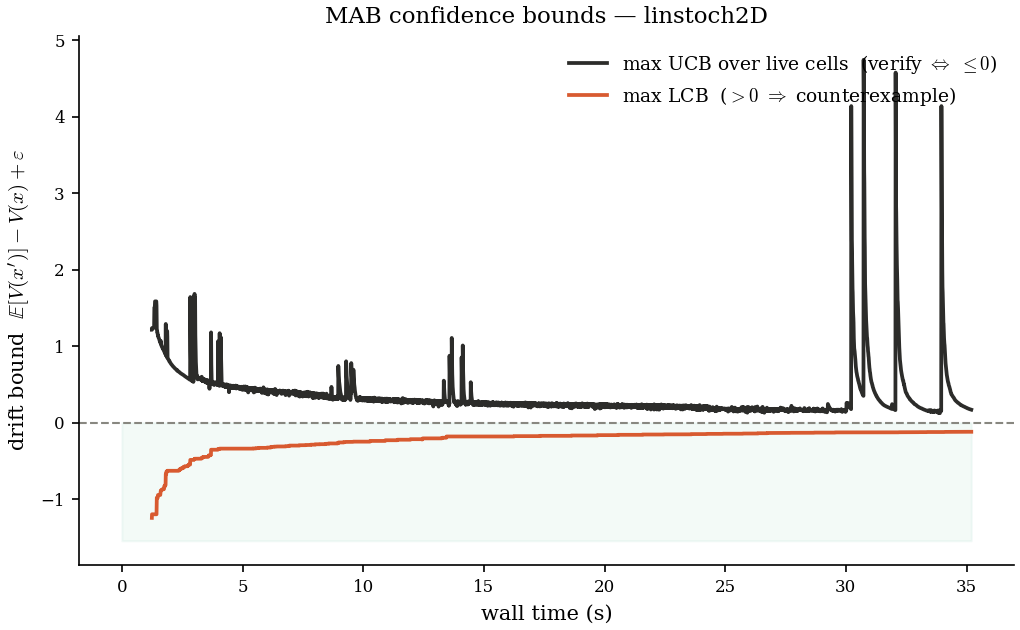
\includegraphics[width=0.49\linewidth]{Figures/mab_bounds.png}
% \caption{The MAB verifier at work on the 2D linear-stochastic certificate.
% \emph{Left:} the fraction of the domain proven safe grows over time as cells are
% retired. \emph{Right:} the global upper and lower confidence bounds on
% $\sup_{x}\drift(x)$ close towards the certification threshold; the run certifies
% once the upper bound falls to $0$. Adaptive refinement concentrates samples on
% the thin-margin frontier, so most of the domain is cleared by a few large
% cells.}
% \label{fig:mab}
% \end{figure}

% \paragraph{Monte Carlo versus MAB.}
% The two sampling verifiers share an interface and a soundness style but sit at
% opposite ends of a cost--precision trade-off. The global Monte Carlo method
% (Algorithm~\ref{alg:mc}) verifies a positive tolerance $\tau$ at cost
% $\sim\tau^{-2(d+1)}$ and can never certify $\tau=0$; a uniform Lipschitz covering
% would already reach $\tau=0$ at cost $\sim(L_{\drift}/\tau_{\mathrm{res}})^d$; and MAB
% (Algorithm~\ref{alg:mab}) attains the same zero-tolerance guarantee while
% spending that exponential cost only where the margin is thin. This progression
% --- global average, uniform cover, adaptive cover --- is precisely the ladder
% that motivates keeping spatial locality in black-box verification.


% \section{Experiments}

% Having described the three verifier families, we ask which of them can actually
% drive certificate synthesis to completion across the benchmark suite, and at
% what cost. We run each engine as the sole verifier in the CEGIS loop --- every
% counterexample is found by the verifier itself --- on the systems of
% Chapter~\ref{chap:benchmarks}, and record whether a valid certificate is reached
% together with the wall-clock and number of CEGIS rounds it takes.

% The result is a capability boundary that follows the dynamics class exactly as
% Chapter~\ref{chap:benchmarks} anticipated (Table~\ref{tab:capability}). The
% \emph{symbolic} engines are the most precise where they apply but the least
% general: Gurobi's MILP encoding is exact yet closes only up to two noise
% dimensions --- the discretisation window shuts by three
% (Figure~\ref{fig:milp_nd}) --- and Z3, though a complete decision procedure for
% the polynomial systems, returned \emph{unknown} or exhausted its budget on
% essentially every trained-network round. Neither can represent the pendulum's
% $\sin\theta$, and both abstain outright. The \emph{sampling} verifiers are the
% most general --- indifferent to the form of the dynamics and the noise --- but
% sound worst-case sampling is costly (Sections~\ref{sec:mc}--\ref{sec:mab}), and
% we were not able to drive it to a full-suite synthesis campaign within budget;
% we report it as a sound-but-expensive method rather than a benchmarked engine.

% \begin{table}[h]
% \centering
% \begin{tabular}{llcccc}
% \hline
% System & Dynamics & Z3 (SMT) & Gurobi (MILP) & LiRPA & MC/MAB \\
% \hline
% Linear (2D) & linear & exact$^\ast$ & exact ($\le$2D) & \checkmark & sound$^\dagger$ \\
% Double-well & polynomial & exact$^\ast$ & exact & \checkmark & sound$^\dagger$ \\
% Pendulum (LQR) & transcendental & abstains & abstains & \checkmark & sound$^\dagger$ \\
% \hline
% \end{tabular}
% \caption{Verifier capability across the suite. \checkmark{} = drives CEGIS to a
% valid certificate. $^\ast$ Z3 is a sound decision procedure for these systems
% but returned \emph{unknown}/timeout on essentially every trained-network round.
% $^\dagger$ the sampling verifiers are sound and general but were not run at
% full-suite scale. The bound-propagation (LiRPA) family is the only one that
% spans the suite, including the transcendental pendulum the symbolic engines
% cannot encode.}
% \label{tab:capability}
% \end{table}

% The bound-propagation (LiRPA) family is the one that spans the suite. IBP, CROWN
% and $\alpha$-CROWN each synthesise a valid certificate on the linear,
% double-well and transcendental-pendulum systems alike --- including the case the
% symbolic engines cannot even encode --- which is what identifies this family as
% the reliable default for stochastic certificate verification. The three engines
% trade per-call tightness against the number of rounds in the expected way, and
% the anytime view in Figure~\ref{fig:pendulum-anytime} makes the trade concrete:
% on a pendulum certificate, IBP's enclosure is the loosest at any compute budget,
% CROWN tightens it, and $\alpha$-CROWN's per-call slope optimisation reaches the
% tightest bound --- but at a steep price, up to $2.7$ hours to certify the
% pendulum in the verifier-only loop (the full verifier-only costs are the
% baseline rows of Table~\ref{tab:cegis-speedup}). That cost, incurred once per
% round and paid mostly on candidates that turn out to be invalid, is exactly what
% the refuter pre-screen of Chapter~\ref{chap:streamlining} removes.

% \begin{figure}[h]
% \centering
% 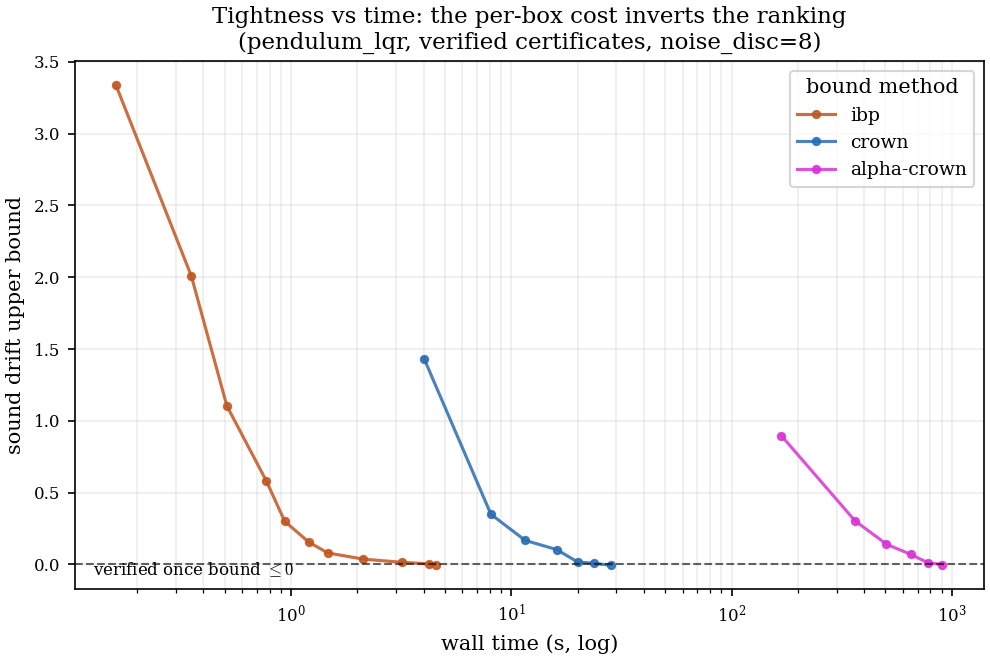
\includegraphics[width=\linewidth]{Figures/pendulum_anytime_time.png}
% \caption{Anytime tightness of the three LiRPA engines on a verified pendulum
% certificate: the certified drift bound against wall-clock as branch-and-bound
% refines. IBP is cheapest per unit compute but loosest; $\alpha$-CROWN reaches
% the tightest bound at the highest cost; CROWN sits between. All three are sound
% at every step (the bound only tightens), the property that lets them be stopped
% early inside the CEGIS loop.}
% \label{fig:pendulum-anytime}
% \end{figure}

% We now turn from the verifiers in isolation to their behaviour inside the full
% synthesis loop, where the dominant cost above --- the sound call on every
% round --- can be pre-empted by a cheap refuter; this is the subject of
% Chapter~\ref{chap:streamlining}.



\newpage


